% ============================================================
%  KUIS 2 — MATEMATIKA (MAE)  T.P. 2026/2027
%  Tema: "LEGO Architecture Challenge" (replika Empire State Building)
%  Bentuk: 1-5 PG Kompleks (Benar/Salah); 6-10 Uraian; 11-12 BONUS
%  Materi inti: Bab 2 Barisan & Deret, Bab 5 SPLTV, Bab 6 Fungsi Kuadrat
%  Prinsip: "progressive blueprint" -> Lembar A..E terbuka bertahap.
%  Data sinkron blueprint: tinggi 55 cm, alas 21 x 13 cm.
%  Kompilasi: pdfLaTeX (gambar berada di folder yang sama)
% ============================================================

\documentclass[11pt]{article}

% ===================== PACKAGES =====================
\usepackage[utf8]{inputenc}
\usepackage[T1]{fontenc}
\usepackage[bahasa]{babel}
\usepackage[a4paper,margin=2.5cm,top=2.8cm]{geometry}
\usepackage{amsmath,amssymb}
\usepackage{graphicx}
\usepackage{tikz}
\usetikzlibrary{arrows.meta}
\usepackage{array}
\usepackage{enumitem}
\usepackage{multicol}
\usepackage{xcolor}
\usepackage[most]{tcolorbox}
\usepackage{fancyhdr}
\usepackage{booktabs}
\usepackage{icomma}

% ===================== HEADER & FOOTER =====================
\pagestyle{fancy}\fancyhf{}
\lhead{\small KUIS 2: Matematika (MAE)}
\rhead{\small T.P. 2026/2027}
\cfoot{\small\thepage}
\renewcommand{\headrulewidth}{0.4pt}

% ===================== KOTAK SOAL =====================
\newtcolorbox{soal}[1]{
  breakable,
  colback=white,
  colframe=black,
  colbacktitle=black,
  coltitle=white,
  fonttitle=\bfseries\sffamily,
  title={Nomor #1},
  boxrule=0.8pt, arc=0pt,
  left=3mm, right=3mm, top=2mm, bottom=2mm}

% ===================== LABEL LEMBAR BLUEPRINT =====================
\newtcolorbox{lembar}[1]{
  colback=blue!4, colframe=blue!45!black, boxrule=0.6pt, arc=1pt,
  left=3mm,right=3mm,top=1.5mm,bottom=1.5mm,
  fonttitle=\bfseries\sffamily\color{white}, coltitle=white,
  colbacktitle=blue!45!black, title={#1}}

% ===================== PILIHAN GANDA KOMPLEKS (Benar/Salah) =====================
\newenvironment{bstabel}{%
  \par\smallskip\begin{center}\renewcommand{\arraystretch}{1.35}%
  \begin{tabular}{@{}p{0.72\textwidth}>{\centering\arraybackslash}m{1.5cm}>{\centering\arraybackslash}m{1.5cm}@{}}
  \toprule
  \textbf{Pernyataan} & \textbf{Benar} & \textbf{Salah}\\\midrule}%
  {\bottomrule\end{tabular}\end{center}}
\newcommand{\bs}[1]{#1 & $\square$ & $\square$\\[1pt]}

% ===================== SUB-SOAL URAIAN (a, b, c, ...) =====================
\newenvironment{subsoal}{%
  \begin{enumerate}[label=\textbf{(\alph*)},leftmargin=1.8em,itemsep=5pt,topsep=3pt]}%
  {\end{enumerate}}

% ===================== GAMBAR =====================
\newcommand{\gambar}[2][0.6\textwidth]{%
  \begin{center}\includegraphics[width=#1]{#2}\end{center}}

\linespread{1.05}

% ===================================================================
%                         ISI DOKUMEN
% ===================================================================
\begin{document}
\thispagestyle{empty}

% ===================== COVER + PETUNJUK (satu halaman) =====================

\begin{center}
  \fbox{\parbox{0.45\textwidth}{\centering\bfseries\large LEMBAR SOAL}}
\end{center}
\vspace{0.4cm}

\begin{center}
  {\LARGE\bfseries KUIS 2: MATEMATIKA (MAE)}\\[0.3em]
  {\large\itshape Studi Kasus \textit{LEGO Architecture Challenge}}
\end{center}
\vspace{0.4cm}

\begin{center}
  \begin{tabular}{@{\hspace{2cm}}ll@{\hspace{0.4cm}:@{\hspace{0.4cm}}}l}
    Jenjang      & & SMA / Madrasah Aliyah \\[0.3em]
    Hari/Tanggal & & [\underline{\hspace{4cm}}] \\[0.3em]
    Waktu        & & 120 menit \\[0.3em]
    Paket Soal   & & -- \\
  \end{tabular}
\end{center}

\vspace{0.4cm}
\noindent\rule{\linewidth}{0.6pt}
\vspace{0.2cm}

\noindent\textbf{\underline{PETUNJUK UMUM}}
\begin{enumerate}[leftmargin=*,itemsep=3pt,topsep=3pt]
  \item Anda \textbf{tidak} diperbolehkan menggunakan sumber eksternal, termasuk
        internet dan \textit{large language model} (ChatGPT, Claude, Gemini, dan
        sebagainya). Kerjakan sendiri, karena kuis ini dibuat untuk
        \textbf{mengukur} tingkat kepahaman Anda.
  \item Soal terdiri atas \textbf{10 butir wajib (Nomor 1--10)} dan \textbf{2 butir
        bonus (Nomor 11--12)}, dan saling \textbf{berkolaborasi}: hasil pada nomor
        awal sering dipakai kembali. Kerjakan \textbf{berurutan}.
  \item Kuis ini memakai \textbf{\textit{progressive blueprint}}: dokumen rancangan
        terbuka bertahap dalam \textbf{Lembar A--E}. \textbf{Banyak data dibaca
        langsung dari lembar (gambar)}: amati skala, kisi brick,
        denah, dan koordinat; angka tidak selalu diberikan dalam teks.
  \item \textbf{Bagian A (Nomor 1--5)} pilihan ganda kompleks (centang
        \textbf{Benar}/\textbf{Salah} tiap pernyataan). \textbf{Bagian B (Nomor
        6--10)} uraian bercabang; proses ikut dinilai.
  \item \textbf{Bagian C (Nomor 11--12): BONUS.} Benar menambah poin; salah/kosong
        tidak mengurangi. Kerjakan hanya jika Nomor 1--10 selesai.
  \item Materi inti: \textbf{Barisan dan Deret} (Bab 2), \textbf{SPLTV} (Bab 5),
        \textbf{Fungsi Kuadrat} (Bab 6), dipadukan dalam kasus rancang-bangun
        menara LEGO.
  \item \textbf{Nilai bantu} (tanpa kalkulator):\\[0.2em]
        \small
        $2^{5}=32$;\ \ $2^{6}=64$;\ \ $15{+}13{+}11{+}9{+}7=55$;\ \
        $80{+}64{+}48{+}32{+}16=240$;\ \ $21\times13=273$;\ \
        $17\times17=289$;\ \ $\sqrt{64}=8$.
  \item Isilah detail berikut.\\[0.3em]
        \textbf{Nama}\hspace{0.45cm};\enspace\underline{\hspace{8cm}}
\end{enumerate}

\vspace{0.3cm}
\noindent\textit{Dengan menandatangani kolom di bawah ini, saya menyatakan telah
membaca, memahami, dan menyetujui seluruh peraturan di atas.}

\vspace{0.4cm}
\noindent\fbox{\parbox{5cm}{\vspace{1.6cm}\centering\small Tanda Tangan Peserta\vspace{0.3cm}}}

\clearpage

% ===================================================================
%                 JUDUL + NARASI (data menyatu di cerita)
% ===================================================================

\begin{center}
  {\Large\bfseries \textit{LEGO Architecture Challenge}: Menara Sang Arsitek Muda}
\end{center}
\vspace{0.3cm}

\begin{center}
  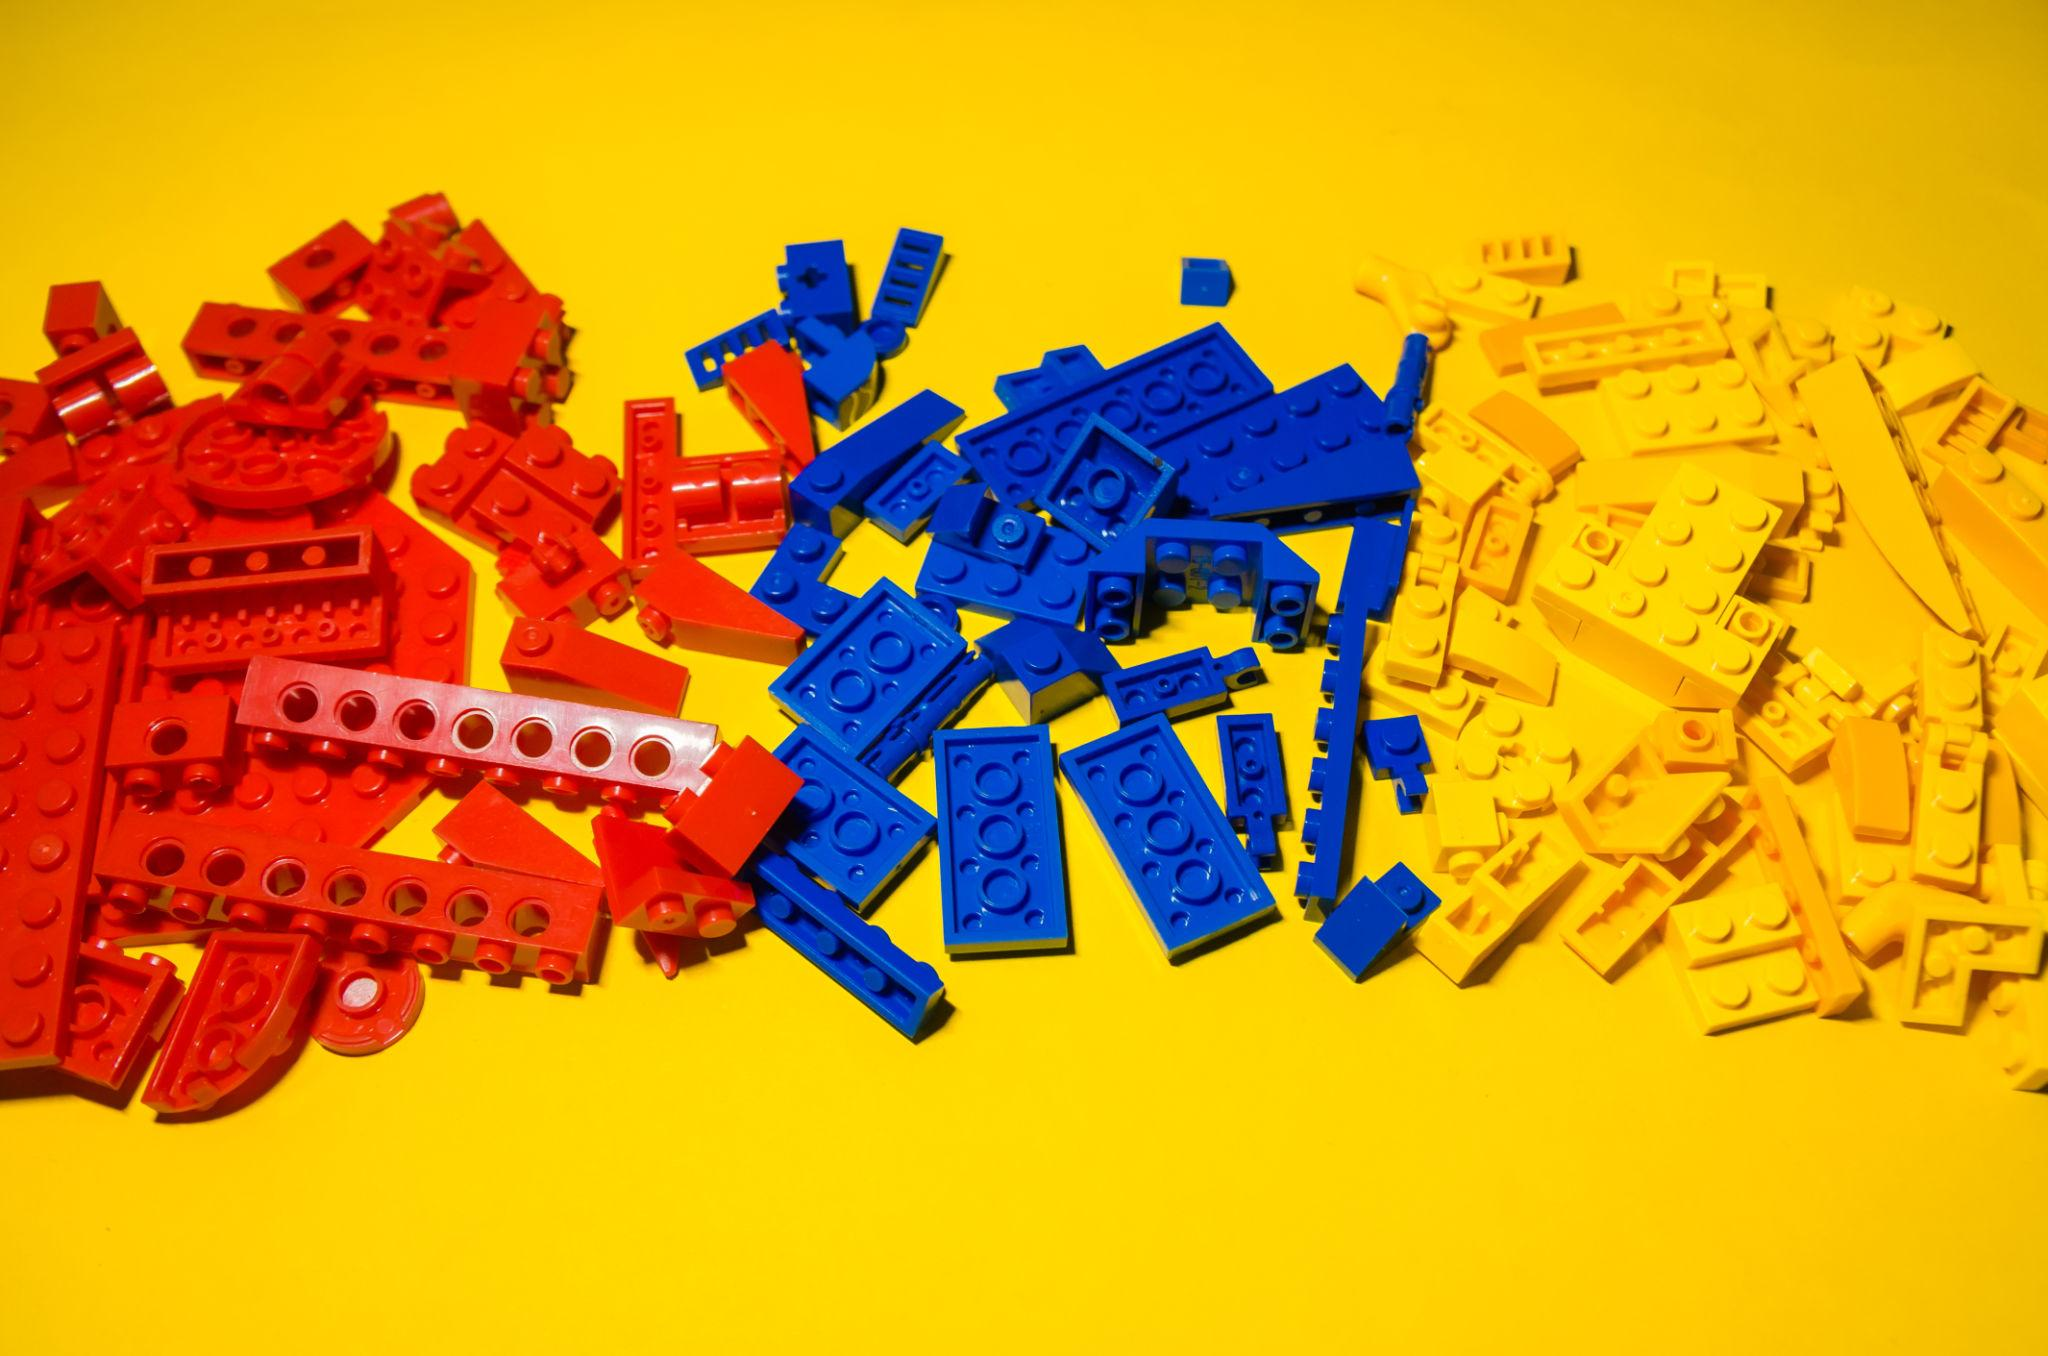
\includegraphics[width=0.6\textwidth]{model-1.jpg}\\[3pt]
  {\small\textit{Tiga jenis brick yang dibagikan panitia: $2\times2$ (merah),
  $2\times4$ (biru), dan $1\times4$ (kuning).}}
\end{center}
\vspace{0.15cm}

Lampu sorot memenuhi aula utama \textbf{LEGO\textsuperscript{\textregistered}
Education Arena}. Di atas ratusan meja putih berjajar tim-tim pelajar dari
seluruh negeri, jantung berdegup menanti aba-aba. Hari itu digelar
\textbf{\textit{LEGO Architecture Challenge}}, kompetisi merancang menara yang
bukan sekadar tinggi, melainkan \emph{cerdas secara matematis}. Panitia tidak
memberi satu gambar utuh; mereka membagikan \textbf{satu map berisi lima lembar
blueprint (Lembar A--E)} yang harus dibuka \emph{bertahap}, persis
seperti seorang arsitek membedah dokumen proyek.

\smallskip
Setiap tim menerima satu kotak berisi \textbf{tepat $240$ brick} dari tiga jenis:
$2\times2$ (merah), $2\times4$ (biru), dan $1\times4$ (kuning). Jumlah tiap
warnanya \emph{tidak} tertera; panitia hanya mencatat \textbf{total massa $500$
gram} dan \textbf{total poin estetika $820$} (rincian pada Lembar B). Dewan juri
menetapkan dua \textbf{syarat estetika}: (i) skor estetika $\ge800$ poin, dan (ii)
proporsi \textbf{brick merah} (warna ciri khas menara) minimal
\textbf{$40\%$} dari seluruh brick.

\smallskip
\textbf{Nendra}, kapten tim ``\textit{Sang Arsitek}'', membuka \textbf{Lembar A}:
replika pencakar langit ikonik bergaya \emph{Empire State}, ramping
\textbf{bertingkat} (\textit{setback}). Tertera ukuran baku yang wajib dicapai:
\textbf{tinggi menara $55$ cm} ($21$ in) dan \textbf{alas $21$ cm $\times$ $13$
cm} ($8$ in $\times$ $5$ in), dengan skala minifigur $1:1$.

\begin{center}
  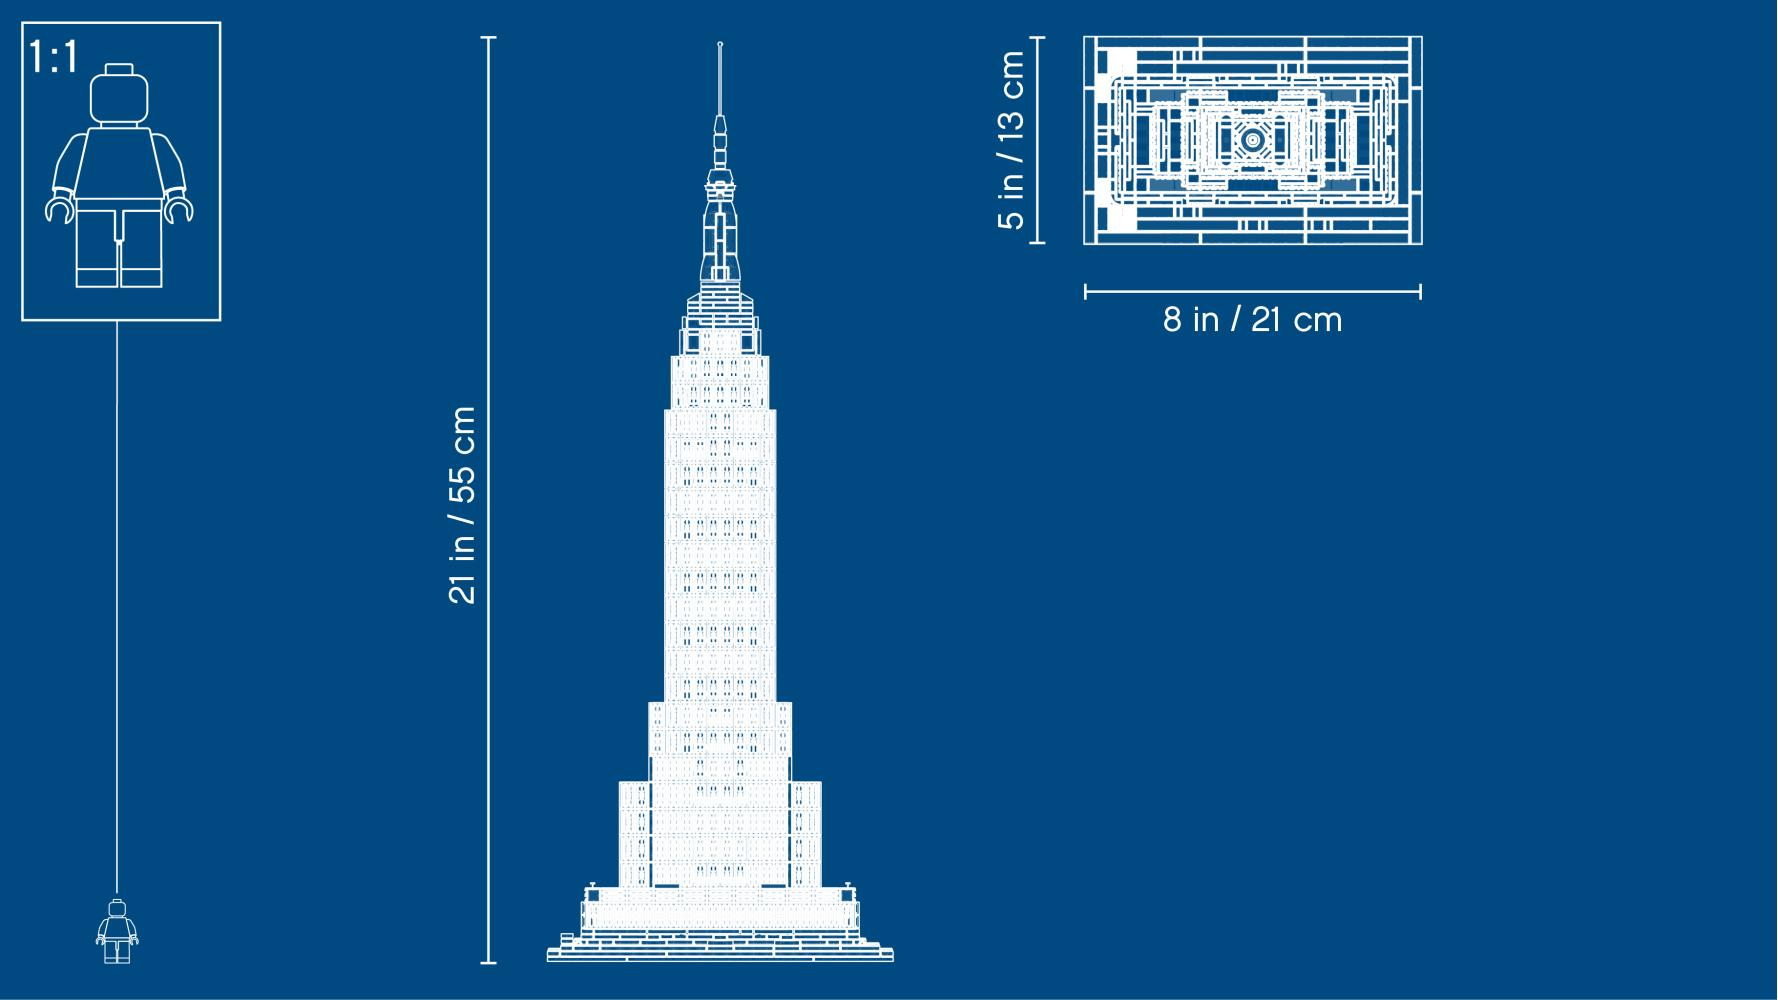
\includegraphics[width=0.9\textwidth]{lego-preview-2.jpg}\\[3pt]
  {\small\textit{Rujukan set resmi: tinggi $55$ cm ($21$ in), alas $21$ cm
  $\times$ $13$ cm ($8\times5$ in), skala minifigur $1:1$.}}
\end{center}

\smallskip
Panitia menegaskan \textbf{empat syarat}: menara harus \textbf{(1) stabil} (denah
tiap tingkat makin sempit ke atas), \textbf{(2) hemat brick} ($240$ terpakai
pas), \textbf{(3) tepat tinggi} ($55$ cm), dan \textbf{(4) estetis} (dua syarat
juri di atas). Badan menara terdiri atas \textbf{$5$ tingkat}. Sentuhan
akhirnya: sebuah \textbf{busur lampu hias LED} melengkung di atas pintu (Lembar
D), dan sebuah \textbf{papan alas} (\textit{base plate}, Lembar E) yang harus
dirancang seluas mungkin. Kemenangan bukan milik yang tercepat, melainkan yang
\textbf{membaca blueprint paling cermat}. Bantu tim ``Sang Arsitek''!

\begin{center}
\begin{tikzpicture}[scale=0.14,font=\footnotesize,>=Latex]
\draw[fill=orange!30,draw=orange!60!black,line width=0.3pt] (-10.5,0)  rectangle (10.5,15);
\draw[fill=orange!30,draw=orange!60!black,line width=0.3pt] (-8.5,15)  rectangle (8.5,28);
\draw[fill=orange!30,draw=orange!60!black,line width=0.3pt] (-6.5,28)  rectangle (6.5,39);
\draw[fill=orange!30,draw=orange!60!black,line width=0.3pt] (-4.5,39)  rectangle (4.5,48);
\draw[fill=orange!30,draw=orange!60!black,line width=0.3pt] (-2.5,48)  rectangle (2.5,55);
\draw[very thick,gray] (0,55)--(0,61);
\draw[thick] (-13,0)--(13,0);
\draw[very thick,blue!55!black,domain=-6:6,samples=40,smooth,variable=\x]
   plot ({\x},{9-0.25*\x*\x});
\node[font=\scriptsize,blue!55!black] at (0,-3){busur lampu LED (Lembar D)};
\draw[<->,red!70!black] (-12.8,0)--(-12.8,55);
\node[left,red!70!black,font=\scriptsize] at (-12.8,27.5){$55$ cm};
\draw[<->,red!70!black] (-10.5,-6.5)--(10.5,-6.5);
\node[below,red!70!black,font=\scriptsize] at (0,-6.6){alas $21$ cm};
\draw[->] (14.5,7.5)--(10.7,7.5);
\node[right,font=\scriptsize] at (14.5,7.5){tingkat ke-$1$ (dasar)};
\draw[->] (14.5,51.5)--(2.7,51.5);
\node[right,font=\scriptsize] at (14.5,51.5){tingkat ke-$5$ (puncak)};
\end{tikzpicture}\\[2pt]
{\small\textbf{Lembar A: Tampak Depan} (tidak berskala). Lima tingkat meruncing
(tinggi total $55$ cm, alas $21$ cm), busur lampu LED di atas pintu. Rincian
tinggi \& brick tiap tingkat dibaca pada Nomor 1--2.}
\end{center}

\vspace{0.3cm}
\noindent\rule{\linewidth}{0.6pt}
\vspace{0.1cm}

\noindent{\large\bfseries BAGIAN A: Pilihan Ganda Kompleks (Nomor 1--5)}\\[0.2em]
\small\emph{Untuk setiap pernyataan, beri tanda centang ($\checkmark$) pada
kolom \textbf{Benar} atau \textbf{Salah}.}\normalsize

\bigskip

% ---------------------------- NOMOR 1 ----------------------------
\begin{soal}{1 \normalfont\itshape(Barisan Aritmetika: baca tinggi dari Lembar A)}
\textbf{Baca tinggi tiap tingkat dari skala pada Lembar A} (garis putus-putus
menunjuk batas atas tiap tingkat pada penggaris cm).

\begin{center}
\begin{tikzpicture}[scale=0.12,font=\scriptsize,>=Latex]
\draw[->,gray](0,0)--(0,60) node[above,font=\tiny]{cm};
\foreach \y in {0,5,10,15,20,25,30,35,40,45,50,55}
  \draw[gray](-0.8,\y)--(0.8,\y) node[left=1pt,font=\tiny] at (-0.8,\y){\y};
\fill[orange!30](4,0)rectangle(20,15);  \draw[orange!60!black,thick](4,0)rectangle(20,15);
\fill[orange!30](5,15)rectangle(19,28); \draw[orange!60!black,thick](5,15)rectangle(19,28);
\fill[orange!30](6,28)rectangle(18,39); \draw[orange!60!black,thick](6,28)rectangle(18,39);
\fill[orange!30](7,39)rectangle(17,48); \draw[orange!60!black,thick](7,39)rectangle(17,48);
\fill[orange!30](8,48)rectangle(16,55); \draw[orange!60!black,thick](8,48)rectangle(16,55);
\foreach \y in {15,28,39,48,55} \draw[dashed,gray](0.8,\y)--(4,\y);
\foreach \mid/\re/\lab in {7.5/20/1, 21.5/19/2, 33.5/18/3, 43.5/17/4, 51.5/16/5}{
  \draw[gray,thin] (\re,\mid)--(23,\mid);
  \node[right,font=\tiny] at (23,\mid){tingkat \lab};}
\end{tikzpicture}
\end{center}
Tentukan Benar/Salah tiap pernyataan (tinggi dalam cm).
\begin{bstabel}
  \bs{(1) Tinggi tingkat membentuk barisan aritmetika dengan beda $d=-2$.}
  \bs{(2) Rumus tinggi tingkat ke-$n$ adalah $a_n=17-2n$.}
  \bs{(3) Tingkat ke-$4$ memiliki tinggi $9$ cm.}
  \bs{(4) Tingkat puncak (ke-$5$) memiliki tinggi $5$ cm.}
\end{bstabel}
\end{soal}

% ---------------------------- NOMOR 2 ----------------------------
\begin{soal}{2 \normalfont\itshape(Deret Aritmetika: hitung brick dari kisi Lembar A)}
Potongan Lembar A berikut memperlihatkan tiap tingkat sebagai \textbf{kisi brick}
($1\times1$ = satu brick). \textbf{Hitung banyak brick tiap tingkat dari kisi.}

\begin{center}
\begin{tikzpicture}[scale=0.2,font=\scriptsize]
\foreach \i/\c/\yb in {1/20/0, 2/16/4, 3/12/8, 4/8/12, 5/4/16}{
  \pgfmathsetmacro{\hw}{\c/2}
  \fill[orange!25] (-\hw,\yb) rectangle (\hw,{\yb+4});
  \draw[step=1,orange!70!black,very thin] (-\hw,\yb) grid (\hw,{\yb+4});
  \draw[orange!60!black,thick] (-\hw,\yb) rectangle (\hw,{\yb+4});
}
\node[right,font=\tiny] at (11,2) {tingkat 1};
\node[right,font=\tiny] at (9,6)  {tingkat 2};
\node[right,font=\tiny] at (7,10) {tingkat 3};
\node[right,font=\tiny] at (5,14) {tingkat 4};
\node[right,font=\tiny] at (3,18) {tingkat 5};
\end{tikzpicture}\\[2pt]
{\small\textit{Kisi brick tiap tingkat (tinggi tidak digambarkan berskala).}}
\end{center}
Tentukan Benar/Salah tiap pernyataan.
\begin{bstabel}
  \bs{(1) Banyak brick tiap tingkat membentuk barisan aritmetika dengan beda $d=-16$.}
  \bs{(2) Jumlah brick pada $3$ tingkat teratas (ke-$3,4,5$) adalah $96$ buah.}
  \bs{(3) Tingkat dasar (ke-$1$) memakai $100$ brick.}
  \bs{(4) Total brick seluruh $5$ tingkat adalah $240$, tepat sama dengan pasokan.}
\end{bstabel}
\end{soal}

% ---------------------------- NOMOR 3 ----------------------------
\begin{soal}{3 \normalfont\itshape(SPLTV: komposisi brick)}
\begin{lembar}{Lembar B: Inventaris Brick}
\small
\renewcommand{\arraystretch}{1.25}
\begin{center}
\begin{tabular}{@{}l >{\centering\arraybackslash}m{2.1cm} c c@{}}
\toprule
\textbf{Jenis} & \textbf{Gambar} & \textbf{Massa} & \textbf{Poin}\\
\midrule
$2\times2$ merah ($x$)  & 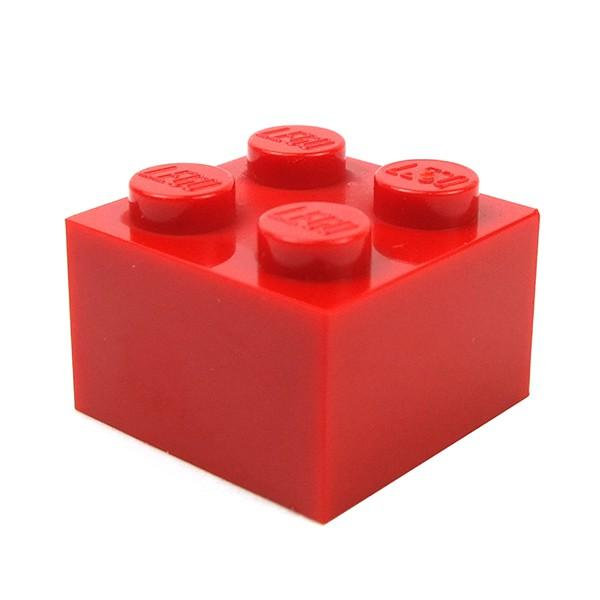
\includegraphics[height=1.05cm]{model-2.jpg} & $2$ g & $3$\\
$2\times4$ biru ($y$)   & 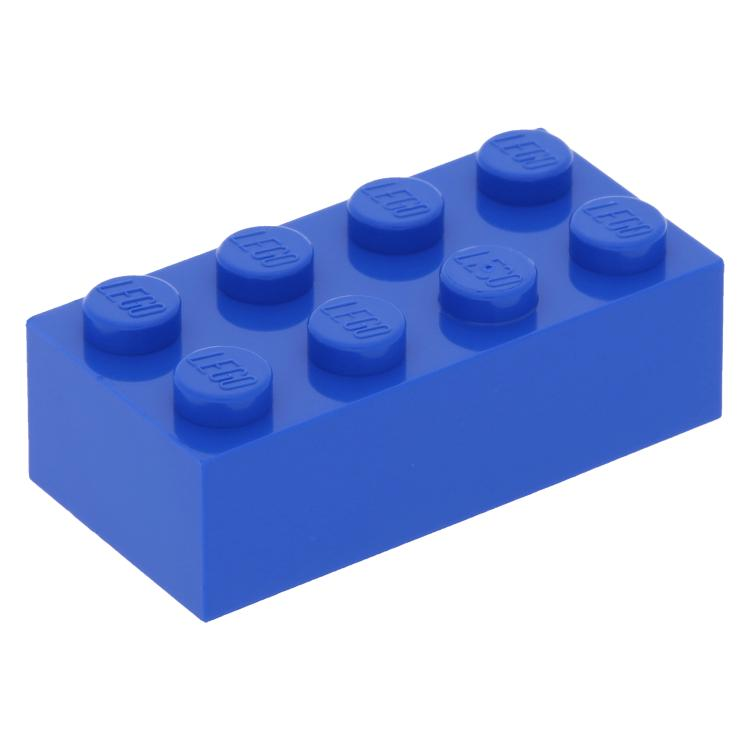
\includegraphics[height=1.05cm]{model-3.jpg} & $3$ g & $5$\\
$1\times4$ kuning ($z$) & 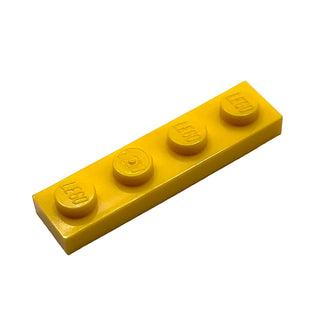
\includegraphics[height=0.9cm]{model-4.jpg} & $1$ g & $2$\\
\midrule
\multicolumn{2}{@{}r}{\textbf{Total:}} & $\mathbf{240}$ brick, $\mathbf{500}$ g & $\mathbf{820}$\\
\bottomrule
\end{tabular}
\end{center}
\textit{Aturan estetika juri:} skor total $\ge800$ poin \textbf{dan} proporsi merah $\ge40\%$.
\end{lembar}

\smallskip
Sebuah tim mengeklaim komposisi brick-nya \textbf{$100$ merah, $80$ biru, $60$
kuning}. \emph{Persamaannya sengaja tidak diberikan}; modelkan sendiri
hubungan jumlah, massa, dan poin dari \textbf{Lembar B}, lalu periksa tiap
pernyataan.
\begin{bstabel}
  \bs{(1) Total brick tim tersebut adalah $240$ buah.}
  \bs{(2) Total massa brick tim tersebut adalah $500$ gram.}
  \bs{(3) Banyak brick biru lebih banyak daripada brick merah.}
  \bs{(4) Total poin estetika brick tim tersebut adalah $820$.}
\end{bstabel}
\end{soal}

% ---------------------------- NOMOR 4 ----------------------------
\begin{soal}{4 \normalfont\itshape(Fungsi Kuadrat: busur lampu LED)}
Tepi busur lampu LED (Lembar D) dimodelkan parabola $y=-\tfrac14 x^2+3x$ (cm).
Tentukan Benar/Salah tiap pernyataan berikut.
\begin{bstabel}
  \bs{(1) Grafik parabola terbuka ke bawah.}
  \bs{(2) Sumbu simetri busur berada di $x=6$.}
  \bs{(3) Tinggi maksimum busur adalah $9$ cm.}
  \bs{(4) Lebar busur di ketinggian tanah (jarak antar kaki) adalah $8$ cm.}
\end{bstabel}
\end{soal}

% ---------------------------- NOMOR 5 ----------------------------
\begin{soal}{5 \normalfont\itshape(Kolaborasi: mencocokkan dengan blueprint)}
Gabungkan hasil Nomor 1--4 dan data blueprint (tinggi $55$ cm, alas $21\times13$
cm, denah tingkat $21,17,13,9,5$ cm). Tentukan Benar/Salah tiap pernyataan.
\begin{bstabel}
  \bs{(1) Jumlah tinggi $5$ tingkat adalah $55$ cm, tepat sesuai blueprint.}
  \bs{(2) Total brick $5$ tingkat ($80{+}64{+}48{+}32{+}16$) adalah $240$.}
  \bs{(3) Alas $21\times13$ cm berbentuk persegi.}
  \bs{(4) Lebar tingkat menurun ($21,17,13,9,5$), tiap tingkat lebih sempit dari bawahnya (stabil).}
\end{bstabel}
\end{soal}

\clearpage
\noindent{\large\bfseries BAGIAN B: Uraian Bercabang (Nomor 6--10)}\\[0.2em]
\small\emph{Kerjakan runtut; tuliskan rumus, substitusi, dan kesimpulan.}\normalsize

\bigskip

% ---------------------------- NOMOR 6 ----------------------------
\begin{soal}{6 \normalfont\itshape(SPLTV: menghitung komposisi brick)}
Gunakan data \textbf{Inventaris Brick (Lembar B, Nomor 3)}: $240$ brick, massa
total $500$ g, poin estetika total $820$. Misalkan $x,y,z$ banyak brick $2\times2$,
$2\times4$, $1\times4$.

\begin{subsoal}
  \item Susun SPLTV dari data jumlah, massa, dan poin estetika.
  \item Dengan eliminasi, hilangkan variabel $z$ sehingga tersisa dua persamaan
        dalam $x$ dan $y$.
  \item Selesaikan sistem dan tentukan $x$, $y$, $z$.
  \item Verifikasi solusi Anda pada ketiga persamaan awal.
  \item Periksa \textbf{syarat estetika juri}: hitung persentase brick merah dan
        simpulkan apakah $\ge40\%$.
\end{subsoal}
\end{soal}

% ---------------------------- NOMOR 7 ----------------------------
\begin{soal}{7 \normalfont\itshape(Barisan \& Deret: analisis revisi blueprint)}
\begin{lembar}{Lembar C: Denah Tampak Atas}
\centering
\begin{tikzpicture}[scale=0.18,font=\scriptsize]
\foreach \w/\d in {21/13, 17/10.5, 13/8, 9/5.5, 5/3}{
  \draw[orange!60!black,fill=orange!12] (-\w/2,-\d/2) rectangle (\w/2,\d/2);
}
\draw[<->,red!70!black] (-10.5,-8.2)--(10.5,-8.2);
\node[below,red!70!black,font=\tiny] at (0,-8.3){lebar terluar $21$ cm};
\end{tikzpicture}\\[2pt]
{\small Denah $5$ tingkat (tampak atas), tersarang: lebar $21,17,13,9,5$ cm;
tiap tingkat menyempit $4$ cm sehingga tumpuan melebar ke bawah (stabil).}
\end{lembar}

\smallskip
Diketahui pola tiap tingkat: \emph{tinggi} $a_1=15$, $d=-2$ (Nomor 1);
\emph{banyak brick} $a_1=80$, $d=-16$ (Nomor 2); \emph{lebar} $a_1=21$, $d=-4$
(Lembar C). Panitia mempertimbangkan \textbf{merevisi} menara.

\begin{subsoal}
  \item Jika menara diperpanjang menjadi \textbf{$8$ tingkat} dengan pola
        \emph{tinggi} yang sama, tentukan tinggi tingkat ke-$8$ dan tinggi total
        $8$ tingkat.
  \item Periksa apakah pola \emph{banyak brick} sanggup mendukung $8$ tingkat.
        Pada tingkat ke berapa pola brick ini mencapai $0$? Apa artinya bagi
        rencana revisi?
  \item Untuk \emph{lebar} tingkat, tentukan rumus suku ke-$n$ dan tunjukkan
        barisannya \textbf{menurun}. Kaitkan dengan \emph{kestabilan} menara.
  \item Lampu LED tiap tingkat membentuk barisan \emph{geometri} $2,4,8,16,32$.
        Tentukan banyak lampu tingkat ke-$5$ dan total lampu seluruh menara. Jika
        tiap LED berdaya $0{,}5$ watt, hitung total daya.
  \item Simpulkan: apakah revisi menjadi $8$ tingkat layak dilakukan? Jelaskan
        berdasarkan hasil (a) dan (b).
\end{subsoal}
\end{soal}

% ---------------------------- NOMOR 8 ----------------------------
\begin{soal}{8 \normalfont\itshape(Fungsi Kuadrat: busur lampu LED)}
\begin{lembar}{Lembar D: Detail Busur Lampu}
\centering
\begin{tikzpicture}[>=Latex,font=\small,xscale=0.42,yscale=0.42]
\draw[help lines,gray!30] (0,0) grid (12,9);
\draw[->,gray] (0,0)--(13.5,0) node[right,font=\scriptsize]{$x$ (cm)};
\draw[->,gray] (0,0)--(0,10.5) node[above,font=\scriptsize]{$y$ (cm)};
\foreach \x in {2,4,6,8,10} \node[below,font=\scriptsize] at (\x,0){\x};
\foreach \y in {3,6,9} \node[left,font=\scriptsize] at (0,\y){\y};
\draw[very thick,blue!55!black,domain=0:12,samples=60,smooth,variable=\x]
   plot ({\x},{-0.25*\x*\x+3*\x});
\fill (0,0) circle(3pt) node[below left,font=\scriptsize]{$(0,0)$};
\fill (12,0) circle(3pt) node[below right,font=\scriptsize]{$(12,0)$};
\draw[dashed,gray] (6,0)--(6,9);
\fill (6,9) circle(3pt) node[above,font=\scriptsize]{puncak $=\,?$};
\end{tikzpicture}\\[2pt]
{\small Busur $y=-\tfrac14 x^2+3x$ (cm); tanah pada $y=0$.}
\end{lembar}

\begin{subsoal}
  \item Tentukan titik potong parabola dengan sumbu-$x$ (kedua kaki busur).
  \item Tentukan persamaan sumbu simetri busur.
  \item Tentukan koordinat titik puncak (tinggi maksimum busur).
  \item Berapa lebar busur di permukaan tanah, dan berapa tinggi maksimumnya?
  \item Untuk memasang papan nama pada ketinggian $y=5$ cm, tentukan lebar busur
        pada ketinggian tersebut.
\end{subsoal}
\end{soal}

% ---------------------------- NOMOR 9 ----------------------------
\begin{soal}{9 \normalfont\itshape(Fungsi Kuadrat: rancangan base plate)}
\begin{lembar}{Lembar E: Rancangan Base Plate}
\centering
\begin{tikzpicture}[scale=0.16,font=\scriptsize]
\draw[orange!60!black,fill=orange!12,thick] (0,0) rectangle (24,14);
\draw[dashed,blue!55!black,thick] (1.5,2) rectangle (22.5,11);
\node[blue!55!black,font=\tiny] at (12,6.5){tapak tingkat-$1$};
\node[below,font=\tiny] at (12,-0.8){lebar tapak $=21$ cm\ ;\ \ base plate: $p+l=34$ cm};
\end{tikzpicture}\\[2pt]
{\small Base plate (garis penuh) harus \emph{memuat} tapak tingkat pertama (garis
putus-putus); tepinya dibingkai brick kuning.}
\end{lembar}

\smallskip
Base plate berbentuk persegi panjang dan harus \textbf{cukup memuat tapak tingkat
pertama} (lebar $21$ cm). Tepinya dibingkai brick kuning sehingga
\textbf{panjang $p$ $+$ lebar $l = 34$ cm}.

\begin{subsoal}
  \item Nyatakan luas base plate $L$ sebagai fungsi panjang $p$.
  \item Tentukan bentuk grafik $L(p)$ dan sumbu simetrinya.
  \item Tentukan $p$ yang memaksimalkan luas beserta luas maksimumnya (abaikan
        dulu syarat memuat menara).
  \item Karena tingkat pertama selebar $21$ cm, sisi panjang \textbf{harus}
        $p\ge21$ cm. Dengan syarat ini, tentukan luas terbesar yang \emph{masih
        dapat memuat menara} beserta ukuran base plate-nya.
  \item Bandingkan hasil (c) dan (d) dengan alas blueprint $21\times13$ cm.
        Jelaskan mengapa blueprint memilih ukuran itu.
\end{subsoal}
\end{soal}

% ---------------------------- NOMOR 10 ----------------------------
\begin{soal}{10 \normalfont\itshape(Kolaborasi: gabungkan seluruh Lembar A--E)}
Gabungkan seluruh lembar blueprint untuk mengambil keputusan akhir: apakah replika
tim ``Sang Arsitek'' memenuhi \textbf{keempat} syarat panitia? Wujud target:
\gambar[0.28\textwidth]{lego-preview-1.jpg}

\begin{subsoal}
  \item \emph{Hemat brick (Lembar A):} bandingkan total brick $5$ tingkat dengan
        pasokan $240$; tentukan sisanya.
  \item \emph{Tepat tinggi (Lembar A):} apakah total tinggi tingkat $=55$ cm?
  \item \emph{Stabil (Lembar C):} dengan lebar $21,17,13,9,5$ cm, jelaskan
        mengapa menara stabil.
  \item \emph{Estetis (Lembar B):} dari $(x,y,z)=(100,80,60)$, hitung total poin
        estetika dan persentase merah; cek kedua syarat juri ($\ge800$ dan
        merah $\ge40\%$).
  \item Simpulkan apakah keempat syarat (hemat, tepat tinggi, stabil, estetis)
        terpenuhi seluruhnya.
\end{subsoal}
\end{soal}

\clearpage
\noindent{\large\bfseries BAGIAN C: Soal Bonus (Nomor 11--12)}\\[0.2em]
\small\emph{Kerjakan hanya bila Nomor 1--10 selesai. Benar menambah poin;
salah/kosong tidak mengurangi.}\normalsize

\bigskip

% ---------------------------- NOMOR 11 (BONUS) ----------------------------
\begin{soal}{11 \normalfont\bfseries[BONUS] \normalfont\itshape(Pola Tersembunyi pada Blueprint)}
Panitia menandai \textbf{empat ukuran kunci} desain (cm) secara berurutan:
\[
13,\quad 21,\quad 34,\quad 55,
\]
yaitu lebar alas, panjang alas, setengah-keliling alas ($21+13$), dan tinggi
menara. Angka-angka ini mengikuti \textbf{satu aturan tersembunyi}.

\begin{subsoal}
  \item Temukan aturan yang menghubungkan keempat bilangan itu, lalu nyatakan
        sebagai hubungan \emph{rekursif} $U_n$ dalam suku-suku sebelumnya.
  \item Dengan aturan itu, tentukan dua bilangan berikutnya ($U_5$ dan $U_6$).
  \item Hitung rasio $\dfrac{21}{13}$, $\dfrac{34}{21}$, $\dfrac{55}{34}$. Apa yang
        Anda amati tentang nilainya?
  \item Bila pola diteruskan, bilangan ke berapa yang \emph{pertama kali} melebihi
        $300$?
\end{subsoal}
\end{soal}

% ---------------------------- NOMOR 12 (BONUS) ----------------------------
\begin{soal}{12 \normalfont\bfseries[BONUS] \normalfont\itshape(SPLTV bertemu Fungsi Kuadrat)}
Panitia mensurvei lengkung atap menara dan mencatat tiga titik yang dilaluinya:
$(0,0)$, $(1,3)$, dan $(2,4)$. Lengkung atap dimodelkan $y=ax^2+bx+c$.

\begin{center}
\begin{tikzpicture}[>=Latex,font=\footnotesize,xscale=0.7,yscale=0.7]
\draw[->,gray] (-0.3,0)--(4.6,0) node[right,font=\scriptsize]{$x$};
\draw[->,gray] (0,-0.3)--(0,5) node[above,font=\scriptsize]{$y$};
\foreach \x in {1,2,3,4} \node[below,font=\scriptsize] at (\x,0){\x};
\foreach \y in {1,2,3,4} \node[left,font=\scriptsize] at (0,\y){\y};
\fill (0,0) circle(2.5pt) node[below left,font=\scriptsize]{$(0,0)$};
\fill (1,3) circle(2.5pt) node[above left,font=\scriptsize]{$(1,3)$};
\fill (2,4) circle(2.5pt) node[above,font=\scriptsize]{$(2,4)$};
\draw[densely dotted,blue!55!black,domain=0:4,samples=40,smooth,variable=\x]
   plot ({\x},{-\x*\x+4*\x});
\end{tikzpicture}\\[2pt]
{\small\textit{Petunjuk:} substitusikan tiap titik ke $y=ax^2+bx+c$.}
\end{center}

\begin{subsoal}
  \item Substitusikan ketiga titik dan susun SPLTV dalam $a$, $b$, $c$.
  \item Selesaikan sistem untuk memperoleh $a$, $b$, $c$.
  \item Tuliskan persamaan lengkung atap.
  \item Tentukan titik puncak atap dan lebar atap (jarak kedua titik potong
        dengan sumbu-$x$).
\end{subsoal}
\end{soal}
\end{document}
